\documentclass[landscape,10pt]{beamer} % use larger type; default would be 10pt
\usepackage{graphicx}
\usepackage{hyperref}
%\usepackage{geometry} % SIVUN DIMENSION MUUTTAMISTA VARTEN
%\geometry{a4paper} % or letterpaper (US) or a5paper or....
%\addtolength{\topmargin}{-.5in} 
\addtolength{\topmargin}{.2cm} 
%\addtolength{\textheight}{1.75in}
%\addtolength{\oddsidemargin}{.1in}
\addtolength{\oddsidemargin}{-.3in}
%\addtolength{\evensidemargin}{-.4in}
\addtolength{\evensidemargin}{-.3in}
\addtolength{\textwidth}{0.6in}
\newcommand{\commentout}[1]{}

\pagestyle{empty}

\begin{document}

\begin{centering}
{. }\\
{. }\\
{. }\\
{. }\\
{. }\\
{. }\\
{. }\\
L3Res global fit status\\
\today\\
Mikko Voutilainen, U. Helsinki and HIP\\
\end{centering}

\newpage

The following slides use inputs from the L3Res team, posted on the (virtual JEC agenda of April 26, 2017 ( \url{https://indico.cern.ch/event/634367/} ) around beginning of May 2017 (up to May 2nd).
These have been processed on top of the \verb|Summer16_03Feb2017H_V2_[DATA/MC]| corrections in the JEC database ({\bf now \verb|V2| for Z+jet also}, and now with {\bf new regression} for $\gamma$+jet), up to \verb|L2Residual| and including new \verb|L1Res|.\\
.\\
I would like to extend special thanks to
\begin{itemize}
\item Alexx Perloff and Sifu Luo for MC truth corrections (L1L2L3)
%\item Bahareh Roozbahani, Charles Harrington and Ia Iashvili for L1Res+L1RC
\item Bahareh Roozbahani and Ia Iashvili for L1Res+L1RC
\item Jens Multhaup and Anastasia Karavdina for L2Res
\item Thomas Berger for Z+jet inputs to L3Res global fit
%\item {\bf Robert Schoefbeck for Z+jet cross-check (shown here)}
\item Hugues Lattaud and Viola Sordini for $\gamma$+jet inputs to L3Res global fit
\item Andrey Popov for multijet inputs to L3Res global fit
\item Hannu Siikonen for valuable checks of the PFJet composition vs $p_T$ and cross-check of the L2Res with single jet triggers
\end{itemize}

\newpage

Some notes about current global fit settings:
\begin{itemize}
\item The electron and muon scales are {\bf not} corrected with the Z mass; this is measured in bins of Z $p_T$ and only a flat constant shift of 0.15\% is seen for both BCDEF and GH, and for ee and $\mu\mu$, at $p_T<400$~GeV
\item The recommended photon scale correction from EGM is applied to input $\gamma$+jet data, with the older $E/p$ measurement in $W$ events by M. Cipriani used for extra uncertainty
%; {\em NB: these two don't seem quite consistent...}
%\item Reverted back to custom photon E/p correction from M. Cipriani, as EGM corrections had issues.
\item The reference scale uncertainties are set to 0.2\% for muons, 0.2\% for electrons, 0.5\% for photons, based on the typical magnitude of the ad-hoc corrections
\item The MPF method is given additional 0.5\% uncertainty for Zee+jet and $\gamma$+jet to cover for possible EM footprint effects
\item JEC parameterization is the 2-p fit already used in Run I; tracker dynamic inefficiency is adequately absorbed in this fit for BCDEF
\item Multijet uncertainties have not been thoroughly revised yet
\end{itemize}

\newpage

The inputs are provided for MPF and $p_T$ balance with $\alpha<0.1, 0.15, 0.20$ and $\alpha<0.3$, the last of which is used for global fit vs $p_T$ and shown separately on the following slides. The other inclusive $\alpha$ bins are used to derive custom FSR+FSR corrections, under the assumption of a linear dependence versus $\alpha$ cut, and log-linear dependence versus $p_T$.

The FSR+ISR corrections are further constrained in the global fit under the assumption that both MPF and $p_T$ balance converge to the same ultimate result (within constraints of their uncorrelated systematics).

\newpage

%Some notes about the results \verb|Summer16_23Sep2016V6[BCD,EF,G,H]|:
Some notes about the results \verb|Summer16_03Feb2016H_V2|:
\begin{itemize}
\item Z+jet and $\gamma$+jet agree well on MC MPF, but differ 2\% on data; Why?
\item Z+jet  and $\gamma$+jet difference on MC $p_T$ balance is due to comparing NLO+PS / multileg (Z+jet) to LO+PS ($\gamma$+jet); Plain Pythia8 overestimates FSR (while Pythia6 in Run I underestimated it)
%\item {\bf they do not agree on data} (at $p_T<300$~GeV)
%\item {\bf they do not agree on MC $p_T$ balance} (Z+jet has odd bump at $p_T\approx 105$~GeV
%\item and therefore result in high $\chi^2$ with large nuisance parameters shifts
%\item As a result, I'm not sure if the global fit result is reliable at $p_T<300$~GeV
%\but Good: Zee+jet and Z$\mu\mu$+jet agree (even on the MC $p_T$ balance humps?)
%\item BCDEF and GH differ significantly due to tracker dynamic inefficiency (TDI)
%; their difference is also confirmed by direct data/data ratio
%\item There is some evidence of EF scale being slightly lower (at most 0.4\%) than BCD; consistent with slightly higher TDI in later higher PU data?
%\item There is some evidence of H at high $p_T$ being slightly lower than G (at most 0.6\%); consistent with HCAL barrel scale dropping with time?
%\item V6 ss done with BCD, EF, G, H breakup for IOVs, but fit and Time uncertainties are derived on the new BCDEFGH combined sample. 
%\item Agreement between Z+jet and $\gamma$+jet samples is the best ever on BCD (and H) for MPF. However, EF and G show large photon footprint effects(?); EMG corrections not era-dependent? BCD dominates BCDEF, while G and H have are of similar size and have opposing effects
%\item $p_T$ balance has unexplained differences between all channels for $\alpha<0.3$, both on data and MC; mystery to be followed up
%\item MC MPF drops far too low at low $p_T$; this could be issue with corrupt MC L1RC (L1FastJet differ between V3 and V6, L1RC do not) spotted by Andrey; data L1FastJet and L1RC did not change between V3 and V6, which could be an issue or not, depending on how L2L3 absorbed changes in L1; However, V6/V4 ratio is stable for MC so L1 likely not the issue, rather the increase in $p_T$ threshold for type-I MET calculation (10~GeV in Run I, 15~GeV in Run II)
%\item Big slope in G and H is something to investigate. Could be affected by not updating L1FastJet for data when L1FastJet for MC was changed? 
\end{itemize}

%\newpage

%\item {\em Some notes about closure inputs:}
%\item {\em Some notes about Summer16 L2ResV5 results:}
%\begin{itemize}
%\item  Z+jet closure plots use MadGraph MC for better statistics in forward region (derivation was aMC@NLO)
%\item Z+jet uses $|\eta|<2.4$ because $|\eta|<1.3$ was missing
%\end{itemize}

%\newpage
%
%\item Observations of BCDEFGH closure using \verb|Summer16_23Sep2016V3|:
%\begin{itemize}
%\item Before global fit, dijet above one for both 0.0--0.8 and 0.8--1.3, both methods (should be at unity for all)
%\item The 0.0-0.8 global fit closure is perfect with $\chi^2/NDF=96.8/90$
%\item The 0.8--1.3 region is shifted down outside uncertainty band. Non-closure driven by both Z+jet and $\gamma$+jet, while before fit within band for dijets
%\item The 2.5--3.0 is over and out for dijets with weird shape, under and out for Z/$\gamma$+jet
%\item For global fit, 2.5--3.0 is ok for fit central value, but $\chi^2/NDF$ is horrible due to large tension between dijet and Z/$\gamma$+jet samples
%\end{itemize}


%\newpage

%\begin{figure}[p]
%\centering
%  \includegraphics[width=0.49\textwidth]{L4/globalFitL3res_orig.pdf}
%  \includegraphics[width=0.49\textwidth]{L4/globalFitL3res_shifted.pdf}
%\caption{Global fit closure test of Sum16V3 IOVs done on combined BCDEFGH sample and $|\eta|<2.4$. The Sum16V3 band is centered aroun 1, with the uncertainty reflecting the latest uncertainties presented in these slides.}
%\end{figure}

%\newpage

%\begin{figure}[p]
%\centering
%  \includegraphics[width=0.49\textwidth]{BCDEFGH/globalFitL3res_orig.pdf}
%  \includegraphics[width=0.49\textwidth]{BCDEFGH/globalFitL3res_shifted.pdf}
%\caption{Global fit done on combined BCDEFGH sample. The Sum16V3 band is centered around a custom BCDEFGH L2L3Res file, with the uncertainty reflecting the latest uncertainties presented in these slides. RelativePt dominates at high $p_T$...}
%\end{figure}

\newpage

\begin{figure}[p]
\centering
%  \includegraphics[width=0.49\textwidth]{BCDEF/globalFitL3res_shifted.pdf}
%  \includegraphics[width=0.49\textwidth]{GH/globalFitL3res_shifted.pdf}
  \includegraphics[width=0.39\textwidth]{BCD/globalFitL3res_shifted.pdf}
  \includegraphics[width=0.39\textwidth]{EF/globalFitL3res_shifted.pdf}\\
  \includegraphics[width=0.39\textwidth]{G/globalFitL3res_shifted.pdf}
  \includegraphics[width=0.39\textwidth]{H/globalFitL3res_shifted.pdf}
%\caption{Left BCDEF, right GH. Different slopes are consistent with tracker dynamic inefficiency present in BCDEF. Both Summer16 fits (black line) are consistently higher at low $p_T$ compared to Spring16 residuals (center of yellow band).}
\end{figure}

\newpage

\begin{figure}[p]
\centering
%  \includegraphics[width=0.49\textwidth]{BCDEF/globalFitL3res_orig.pdf}
%  \includegraphics[width=0.49\textwidth]{GH/globalFitL3res_orig.pdf}
  \includegraphics[width=0.39\textwidth]{BCD/globalFitL3res_orig.pdf}
  \includegraphics[width=0.39\textwidth]{EF/globalFitL3res_orig.pdf}\\
  \includegraphics[width=0.39\textwidth]{G/globalFitL3res_orig.pdf}
  \includegraphics[width=0.39\textwidth]{H/globalFitL3res_orig.pdf}
\end{figure}

\newpage

\begin{figure}[p]
\centering
%  \includegraphics[width=0.49\textwidth]{BCDEF/globalFitL3res_raw.pdf}
%  \includegraphics[width=0.49\textwidth]{GH/globalFitL3res_raw.pdf}
  \includegraphics[width=0.39\textwidth]{BCD/globalFitL3res_raw.pdf}
  \includegraphics[width=0.39\textwidth]{EF/globalFitL3res_raw.pdf}\\
  \includegraphics[width=0.39\textwidth]{G/globalFitL3res_raw.pdf}
  \includegraphics[width=0.39\textwidth]{H/globalFitL3res_raw.pdf}
%\caption{Left BCDEF, right GH. Different slopes are consistent with tracker dynamic inefficiency present in BCDEF. Both Summer16 fits (black line) are consistently higher at low $p_T$ compared to Spring16 residuals (center of yellow band).}
\end{figure}

\commentout{

\newpage

\begin{figure}[p]
\centering
  \includegraphics[width=0.49\textwidth]{../test/pdf/compareJECversions_AK4PFchs_MC_L1_Sum16overSpr16.pdf}
  \includegraphics[width=0.49\textwidth]{../test/pdf/compareJECversions_AK4PFchs_DATA_L1_Sum16overSpr16.pdf}
\caption{Left is L1 correction for MC, right is for data (L1*L1Res).}
\end{figure}

\newpage

\begin{figure}[p]
\centering
  \includegraphics[width=0.49\textwidth]{../test/pdf/compareJECversions_AK4PFchs_DATA_L2L3_Sum16overSpr16.pdf}
  \includegraphics[width=0.49\textwidth]{../test/pdf/compareJECversions_AK4PFchs_DATA_L1L2L3_Sum16overSpr16.pdf}
\caption{Left is ratio of MC truth correction, right also includes L1\_Data. Change in L3Res $p_T$ dependence is correlated with the offset correction.}
\end{figure}

\newpage

\begin{figure}[p]
\centering
  \includegraphics[width=0.49\textwidth]{../test/pdf/compareJECversions_AK4PFchs_DATA_L1_Sum16overSpr16.pdf}
  \includegraphics[width=0.49\textwidth]{../test/pdf/compareJECversions_AK4PFchs_DATA_L2L3PlusL2L3Res_Sum16overSpr16.pdf}
\caption{Left is L1 correction, right is L2L3+Res for data.}
\end{figure}

\newpage

\begin{figure}[p]
\centering
  \includegraphics[width=0.49\textwidth]{../test/pdf/compareJECversions_AK4PFchs_DATA_L2L3Res_Sum16overSpr16.pdf}
  \includegraphics[width=0.49\textwidth]{../test/pdf/compareJECversions_AK4PFchs_DATA_L1L2L3PlusL2L3Res_Sum16overSpr16.pdf}
\caption{Left is L2L3Res correction, right is all correction levels for data.}
\end{figure}

} % commentout

\newpage

\begin{figure}[p]
\centering
  \includegraphics[width=0.33\textwidth]{BCD/globalFitL3res_raw.pdf}
  \includegraphics[width=0.33\textwidth]{BCD/globalFitL3res_orig.pdf}
  \includegraphics[width=0.33\textwidth]{BCD/globalFitL3res_shifted.pdf}
\end{figure}
\begin{figure}[p]
\centering
  \includegraphics[width=0.33\textwidth]{BCD/globalFitL3res_hsrc.pdf}
  \includegraphics[width=0.33\textwidth]{BCD/globalFitL3res_mpfchs1_kfsr.pdf}
  \includegraphics[width=0.33\textwidth]{BCD/globalFitL3res_ptchs_kfsr.pdf}
\end{figure}

\newpage

\begin{figure}[p]
\centering
  \includegraphics[width=0.33\textwidth]{EF/globalFitL3res_raw.pdf}
  \includegraphics[width=0.33\textwidth]{EF/globalFitL3res_orig.pdf}
  \includegraphics[width=0.33\textwidth]{EF/globalFitL3res_shifted.pdf}
\end{figure}
\begin{figure}[p]
\centering
  \includegraphics[width=0.33\textwidth]{EF/globalFitL3res_hsrc.pdf}
  \includegraphics[width=0.33\textwidth]{EF/globalFitL3res_mpfchs1_kfsr.pdf}
  \includegraphics[width=0.33\textwidth]{EF/globalFitL3res_ptchs_kfsr.pdf}
\end{figure}

\newpage

\commentout{
\begin{figure}[p]
\centering
  \includegraphics[width=0.33\textwidth]{BCDEFGH/globalFitL3res_raw.pdf}
  \includegraphics[width=0.33\textwidth]{BCDEFGH/globalFitL3res_orig.pdf}
  \includegraphics[width=0.33\textwidth]{BCDEFGH/globalFitL3res_shifted.pdf}
\end{figure}
\begin{figure}[p]
\centering
  \includegraphics[width=0.33\textwidth]{BCDEFGH/globalFitL3res_hsrc.pdf}
  \includegraphics[width=0.33\textwidth]{BCDEFGH/globalFitL3res_mpfchs1_kfsr.pdf}
  \includegraphics[width=0.33\textwidth]{BCDEFGH/globalFitL3res_ptchs_kfsr.pdf}
\end{figure}

\newpage
} %commentout

\begin{figure}[p]
\centering
  \includegraphics[width=0.33\textwidth]{G/globalFitL3res_raw.pdf}
  \includegraphics[width=0.33\textwidth]{G/globalFitL3res_orig.pdf}
  \includegraphics[width=0.33\textwidth]{G/globalFitL3res_shifted.pdf}
\end{figure}
\begin{figure}[p]
\centering
  \includegraphics[width=0.33\textwidth]{G/globalFitL3res_hsrc.pdf}
  \includegraphics[width=0.33\textwidth]{G/globalFitL3res_mpfchs1_kfsr.pdf}
  \includegraphics[width=0.33\textwidth]{G/globalFitL3res_ptchs_kfsr.pdf}
\end{figure}

\newpage

\begin{figure}[p]
\centering
  \includegraphics[width=0.33\textwidth]{H/globalFitL3res_raw.pdf}
  \includegraphics[width=0.33\textwidth]{H/globalFitL3res_orig.pdf}
  \includegraphics[width=0.33\textwidth]{H/globalFitL3res_shifted.pdf}
\end{figure}
\begin{figure}[p]
\centering
  \includegraphics[width=0.33\textwidth]{H/globalFitL3res_hsrc.pdf}
  \includegraphics[width=0.33\textwidth]{H/globalFitL3res_mpfchs1_kfsr.pdf}
  \includegraphics[width=0.33\textwidth]{H/globalFitL3res_ptchs_kfsr.pdf}
\end{figure}

\newpage

\begin{figure}[p]
\centering
  \includegraphics[width=0.33\textwidth]{Sum16V4/H/globalFitL3res_raw.pdf}
  \includegraphics[width=0.33\textwidth]{Sum16V4/H/globalFitL3res_orig.pdf}
  \includegraphics[width=0.33\textwidth]{Sum16V4/H/globalFitL3res_shifted.pdf}
\end{figure}
\begin{figure}[p]
\centering
  \includegraphics[width=0.33\textwidth]{Sum16V4/H/globalFitL3res_hsrc.pdf}
  \includegraphics[width=0.33\textwidth]{Sum16V4/H/globalFitL3res_mpfchs1_kfsr.pdf}
  \includegraphics[width=0.33\textwidth]{Sum16V4/H/globalFitL3res_ptchs_kfsr.pdf}
\end{figure}

\commentout{
\newpage

\begin{figure}[p]
\centering
  \includegraphics[width=0.33\textwidth]{L4/globalFitL3res_raw.pdf}
  \includegraphics[width=0.33\textwidth]{L4/globalFitL3res_orig.pdf}
  \includegraphics[width=0.33\textwidth]{L4/globalFitL3res_shifted.pdf}
\end{figure}
\begin{figure}[p]
\centering
  \includegraphics[width=0.33\textwidth]{L4/globalFitL3res_hsrc.pdf}
  \includegraphics[width=0.33\textwidth]{L4/globalFitL3res_mpfchs1_kfsr.pdf}
  \includegraphics[width=0.33\textwidth]{L4/globalFitL3res_ptchs_kfsr.pdf}
\end{figure}
}% commentout

\commentout{
\newpage

\begin{figure}[p]
\centering
\includegraphics[width=0.33\textwidth]{drawBCDEFvsGH_mpfchs1_ptchs.pdf}
\includegraphics[width=0.33\textwidth]{drawEFvsBCD_mpfchs1_ptchs.pdf}
\includegraphics[width=0.33\textwidth]{drawHvsG_mpfchs1_ptchs.pdf}\\
\includegraphics[width=0.33\textwidth]{drawBCDEFvsGH_mpfchs1_ptchs_nogjmpf_mjvsjes.pdf}
\includegraphics[width=0.33\textwidth]{drawEFvsBCD_mpfchs1_ptchs_nogjmpf.pdf}
\includegraphics[width=0.33\textwidth]{drawHvsG_mpfchs1_ptchs_nogjmpf.pdf}
\end{figure}
} % commentout

\newpage

\begin{figure}[p]
\centering
  \includegraphics[width=1.00\textwidth]{BCD/softrad_2x6_vspt.pdf}
\end{figure}

\newpage

\begin{figure}[p]
\centering
  \includegraphics[width=0.33\textwidth]{BCD/paper_softrad_data_mpfchs1_vspt.pdf}
  \includegraphics[width=0.33\textwidth]{BCD/paper_softrad_mc_mpfchs1_vspt.pdf}
  \includegraphics[width=0.33\textwidth]{BCD/paper_softrad_ratio_mpfchs1_vspt.pdf}
\end{figure}

\begin{figure}[p]
\centering
  \includegraphics[width=0.33\textwidth]{BCD/paper_softrad_data_ptchs_vspt.pdf}
  \includegraphics[width=0.33\textwidth]{BCD/paper_softrad_mc_ptchs_vspt.pdf}
  \includegraphics[width=0.33\textwidth]{BCD/paper_softrad_ratio_ptchs_vspt.pdf}
\end{figure}

\newpage

\begin{figure}[p]
\centering
  \includegraphics[width=0.33\textwidth]{EF/paper_softrad_data_mpfchs1_vspt.pdf}
  \includegraphics[width=0.33\textwidth]{EF/paper_softrad_mc_mpfchs1_vspt.pdf}
  \includegraphics[width=0.33\textwidth]{EF/paper_softrad_ratio_mpfchs1_vspt.pdf}
\end{figure}

\begin{figure}[p]
\centering
  \includegraphics[width=0.33\textwidth]{EF/paper_softrad_data_ptchs_vspt.pdf}
  \includegraphics[width=0.33\textwidth]{EF/paper_softrad_mc_ptchs_vspt.pdf}
  \includegraphics[width=0.33\textwidth]{EF/paper_softrad_ratio_ptchs_vspt.pdf}
\end{figure}

\commentout{
\newpage

\begin{figure}[p]
\centering
  \includegraphics[width=0.33\textwidth]{BCDEFGH/paper_softrad_data_mpfchs1_vspt.pdf}
  \includegraphics[width=0.33\textwidth]{BCDEFGH/paper_softrad_mc_mpfchs1_vspt.pdf}
  \includegraphics[width=0.33\textwidth]{BCDEFGH/paper_softrad_ratio_mpfchs1_vspt.pdf}
\end{figure}

\begin{figure}[p]
\centering
  \includegraphics[width=0.33\textwidth]{BCDEFGH/paper_softrad_data_ptchs_vspt.pdf}
  \includegraphics[width=0.33\textwidth]{BCDEFGH/paper_softrad_mc_ptchs_vspt.pdf}
  \includegraphics[width=0.33\textwidth]{BCDEFGH/paper_softrad_ratio_ptchs_vspt.pdf}
\end{figure}
} %commentout


\newpage
\commentout{
\begin{figure}[p]
\centering
  \includegraphics[width=0.33\textwidth]{L4/paper_softrad_data_mpfchs1_vspt.pdf}
  \includegraphics[width=0.33\textwidth]{L4/paper_softrad_mc_mpfchs1_vspt.pdf}
  \includegraphics[width=0.33\textwidth]{L4/paper_softrad_ratio_mpfchs1_vspt.pdf}
\end{figure}

\begin{figure}[p]
\centering
  \includegraphics[width=0.33\textwidth]{L4/paper_softrad_data_ptchs_vspt.pdf}
  \includegraphics[width=0.33\textwidth]{L4/paper_softrad_mc_ptchs_vspt.pdf}
  \includegraphics[width=0.33\textwidth]{L4/paper_softrad_ratio_ptchs_vspt.pdf}
\end{figure}
} %commentout

\newpage

\begin{figure}[p]
\centering
  \includegraphics[width=0.31\textwidth]{compareJECdata_JME100vsSum16V4_data_gamjet_mpfchs1_a30.pdf}
  \includegraphics[width=0.31\textwidth]{compareJECdata_JME100vsSum16V4_mc_gamjet_mpfchs1_a30.pdf}
  \includegraphics[width=0.31\textwidth]{compareJECdata_JME100vsSum16V4_ratio_gamjet_mpfchs1_a30.pdf}
%\end{figure}
\\
%\begin{figure}[p]
\centering
  \includegraphics[width=0.31\textwidth]{compareJECdata_JME100vsSum16V4_data_gamjet_ptchs_a30.pdf}
  \includegraphics[width=0.31\textwidth]{compareJECdata_JME100vsSum16V4_mc_gamjet_ptchs_a30.pdf}
  \includegraphics[width=0.31\textwidth]{compareJECdata_JME100vsSum16V4_ratio_gamjet_ptchs_a30.pdf}
\end{figure}

\newpage

\begin{figure}[p]
\centering
  \includegraphics[width=0.33\textwidth]{G/paper_softrad_data_mpfchs1_vspt.pdf}
  \includegraphics[width=0.33\textwidth]{G/paper_softrad_mc_mpfchs1_vspt.pdf}
  \includegraphics[width=0.33\textwidth]{G/paper_softrad_ratio_mpfchs1_vspt.pdf}
\end{figure}

\begin{figure}[p]
\centering
  \includegraphics[width=0.33\textwidth]{G/paper_softrad_data_ptchs_vspt.pdf}
  \includegraphics[width=0.33\textwidth]{G/paper_softrad_mc_ptchs_vspt.pdf}
  \includegraphics[width=0.33\textwidth]{G/paper_softrad_ratio_ptchs_vspt.pdf}
\end{figure}

\newpage

\begin{figure}[p]
\centering
  \includegraphics[width=0.33\textwidth]{H/paper_softrad_data_mpfchs1_vspt.pdf}
  \includegraphics[width=0.33\textwidth]{H/paper_softrad_mc_mpfchs1_vspt.pdf}
  \includegraphics[width=0.33\textwidth]{H/paper_softrad_ratio_mpfchs1_vspt.pdf}
\end{figure}

\begin{figure}[p]
\centering
  \includegraphics[width=0.33\textwidth]{H/paper_softrad_data_ptchs_vspt.pdf}
  \includegraphics[width=0.33\textwidth]{H/paper_softrad_mc_ptchs_vspt.pdf}
  \includegraphics[width=0.33\textwidth]{H/paper_softrad_ratio_ptchs_vspt.pdf}
\end{figure}

\newpage

\begin{figure}[p]
\centering
  \includegraphics[width=0.33\textwidth]{Sum16V4/H/paper_softrad_data_mpfchs1_vspt.pdf}
  \includegraphics[width=0.33\textwidth]{Sum16V4/H/paper_softrad_mc_mpfchs1_vspt.pdf}
  \includegraphics[width=0.33\textwidth]{Sum16V4/H/paper_softrad_ratio_mpfchs1_vspt.pdf}
\end{figure}

\begin{figure}[p]
\centering
  \includegraphics[width=0.33\textwidth]{Sum16V4/H/paper_softrad_data_ptchs_vspt.pdf}
  \includegraphics[width=0.33\textwidth]{Sum16V4/H/paper_softrad_mc_ptchs_vspt.pdf}
  \includegraphics[width=0.33\textwidth]{Sum16V4/H/paper_softrad_ratio_ptchs_vspt.pdf}
\end{figure}

\newpage

\begin{figure}[p]
\centering
  \includegraphics[width=0.33\textwidth]{J/paper_softrad_data_mpfchs1_vspt.pdf}
  \includegraphics[width=0.33\textwidth]{J/paper_softrad_mc_mpfchs1_vspt.pdf}
  \includegraphics[width=0.33\textwidth]{J/paper_softrad_ratio_mpfchs1_vspt.pdf}
\end{figure}

\begin{figure}[p]
\centering
  \includegraphics[width=0.33\textwidth]{J/paper_softrad_data_ptchs_vspt.pdf}
  \includegraphics[width=0.33\textwidth]{J/paper_softrad_mc_ptchs_vspt.pdf}
  \includegraphics[width=0.33\textwidth]{J/paper_softrad_ratio_ptchs_vspt.pdf}
\end{figure}

\newpage

%%%%%%%%%%%%%%%%%%%%%%%%%%%%%%%%%%%%%%%%%%%%%%%%%%%%%%%%%%%%
%%%%%%%%%%%%%%%%%  Systematics  %%%%%%%%%%%%%%%%%%%%%%%%%%%%
%%%%%%%%%%%%%%%%%%%%%%%%%%%%%%%%%%%%%%%%%%%%%%%%%%%%%%%%%%%%
\commentout{
\begin{figure}[p]
\centering
\includegraphics[width=0.33\textwidth]{J/JECUncert_DATA_Summary_AK5PFchs_Eta00}
\includegraphics[width=0.33\textwidth]{J/JECUncert_DATA_Summary_AK5PFchs_Eta27}
\includegraphics[width=0.33\textwidth]{J/JECUncert_DATA_Summary_AK5PFchs_Eta35}\\
\includegraphics[width=0.33\textwidth]{J/JECUncert_DATA_Summary_AK5PFchs_Pt30}
\includegraphics[width=0.33\textwidth]{J/JECUncert_DATA_Summary_AK5PFchs_Pt100}
\includegraphics[width=0.33\textwidth]{J/JECUncert_DATA_Summary_AK5PFchs_Pt1000}
\end{figure}

\newpage

\begin{figure}[p]
\centering
  \includegraphics[width=0.33\textwidth]{JECUncert_DATA_Summary_AK4PFchs_Eta00}
  \includegraphics[width=0.33\textwidth]{JECUncert_DATA_Summary_AK4PFchs_Eta27}
  \includegraphics[width=0.33\textwidth]{JECUncert_DATA_Summary_AK4PFchs_Eta35}\\
  \includegraphics[width=0.33\textwidth]{JECUncert_DATA_Summary_AK4PFchs_Pt30}
  \includegraphics[width=0.33\textwidth]{JECUncert_DATA_Summary_AK4PFchs_Pt100}
  \includegraphics[width=0.33\textwidth]{JECUncert_DATA_Summary_AK4PFchs_Pt1000}
\end{figure}

\newpage

\begin{figure}[p]
\centering
  \includegraphics[width=0.33\textwidth]{J/JECUncert_PileUp_AK5PFchs_Pt30}
  \includegraphics[width=0.33\textwidth]{J/JECUncert_PileUp_AK5PFchs_Eta00}\\
  \includegraphics[width=0.33\textwidth]{J/JECUncert_PileUp_AK5PFchs_Eta27}
  \includegraphics[width=0.33\textwidth]{J/JECUncert_PileUp_AK5PFchs_Eta35}
\end{figure}

\newpage

\begin{figure}[p]
\centering
  \includegraphics[width=0.33\textwidth]{JECUncert_PileUp_AK4PFchs_Pt30}
  \includegraphics[width=0.33\textwidth]{JECUncert_PileUp_AK4PFchs_Eta00}\\
  \includegraphics[width=0.33\textwidth]{JECUncert_PileUp_AK4PFchs_Eta27}
  \includegraphics[width=0.33\textwidth]{JECUncert_PileUp_AK4PFchs_Eta35}
\end{figure}

\newpage

\begin{figure}[p]
\centering
  \includegraphics[width=0.33\textwidth]{J/JECUncert_Relative_AK5PFchs_Pt30}
  \includegraphics[width=0.33\textwidth]{J/JECUncert_Relative_AK5PFchs_Pt100}
  \includegraphics[width=0.33\textwidth]{J/JECUncert_Relative_AK5PFchs_Eta27}\\
  \includegraphics[width=0.33\textwidth]{J/JECSource_Time_AK5PFchs_Pt30}
  \includegraphics[width=0.33\textwidth]{J/JECSource_Time_AK5PFchs_Eta00}
  \includegraphics[width=0.33\textwidth]{J/JECSource_AbsolutePt_AK5PFchs_Eta00}
\end{figure}

\newpage 

\begin{figure}[p]
\centering
  \includegraphics[width=0.33\textwidth]{JECUncert_Relative_AK4PFchs_Pt30}
  \includegraphics[width=0.33\textwidth]{JECUncert_Relative_AK4PFchs_Pt100}
  \includegraphics[width=0.33\textwidth]{JECUncert_Relative_AK4PFchs_Eta27}\\
  \includegraphics[width=0.33\textwidth]{JECUncert_Time_AK4PFchs_Pt30}
  \includegraphics[width=0.33\textwidth]{JECUncert_Time_AK4PFchs_Eta00}
  \includegraphics[width=0.33\textwidth]{JECUncert_AbsolutePt_AK4PFchs_Eta00}
\end{figure}

\newpage

\begin{figure}[p]
\centering
  \includegraphics[width=0.33\textwidth]{JECUncert_Relative_AK4PFchs_Pt30}
  \includegraphics[width=0.33\textwidth]{JECUncert_Relative_AK4PFchs_Pt100}
  \includegraphics[width=0.33\textwidth]{JECUncert_Relative_AK4PFchs_Pt500}\\
  \includegraphics[width=0.33\textwidth]{JECUncert_Time_AK4PFchs_Pt30}
  \includegraphics[width=0.33\textwidth]{JECUncert_Time_AK4PFchs_Pt100}
  \includegraphics[width=0.33\textwidth]{JECUncert_Time_AK4PFchs_Pt500}
\end{figure}

\newpage

\begin{figure}[p]
\centering
\includegraphics[width=0.33\textwidth]{J/JECSource_Flavor_AK5PFchs_Eta00}
\includegraphics[width=0.33\textwidth]{J/JECSource_Flavor_AK5PFchs_Eta27}\\
\includegraphics[width=0.33\textwidth]{J/JECSource_Flavor_AK5PFchs_Pt30}
\includegraphics[width=0.33\textwidth]{J/JECSource_Flavor_AK5PFchs_Pt100}
\end{figure}

\newpage
\begin{figure}[p]
\centering
\includegraphics[width=0.33\textwidth]{JECSource_Flavor_AK4PFchs_Eta00}
\includegraphics[width=0.33\textwidth]{JECSource_Flavor_AK4PFchs_Eta27}\\
\includegraphics[width=0.33\textwidth]{JECSource_Flavor_AK4PFchs_Pt30}
\includegraphics[width=0.33\textwidth]{JECSource_Flavor_AK4PFchs_Pt100}
\end{figure}

\newpage

\begin{figure}[p]
\centering
%  \includegraphics[width=0.24\textwidth]{L4/globalFitL3res_orig.pdf}
  \includegraphics[width=0.33\textwidth]{L4/globalFitL3res_raw_eta0-8.pdf}
  \includegraphics[width=0.33\textwidth]{L4/globalFitL3res_raw_eta8-13.pdf}
  \includegraphics[width=0.33\textwidth]{L4/globalFitL3res_raw_eta13-19.pdf}
\end{figure}
\begin{figure}[p]
\centering
  \includegraphics[width=0.33\textwidth]{L4/globalFitL3res_raw_eta19-25.pdf}
  \includegraphics[width=0.33\textwidth]{L4/globalFitL3res_raw_eta25-30.pdf}
%  \includegraphics[width=0.24\textwidth]{L4/globalFitL3res_raw_eta30-32.pdf}
  \includegraphics[width=0.33\textwidth]{L4/globalFitL3res_raw_eta32-52.pdf}
\end{figure}

\newpage

\begin{figure}[p]
\centering
%  \includegraphics[width=0.24\textwidth]{L4/globalFitL3res_orig.pdf}
  \includegraphics[width=0.33\textwidth]{L4/globalFitL3res_orig_eta0-8.pdf}
  \includegraphics[width=0.33\textwidth]{L4/globalFitL3res_orig_eta8-13.pdf}
  \includegraphics[width=0.33\textwidth]{L4/globalFitL3res_orig_eta13-19.pdf}
\end{figure}
\begin{figure}[p]
\centering
  \includegraphics[width=0.33\textwidth]{L4/globalFitL3res_orig_eta19-25.pdf}
  \includegraphics[width=0.33\textwidth]{L4/globalFitL3res_orig_eta25-30.pdf}
%  \includegraphics[width=0.24\textwidth]{L4/globalFitL3res_orig_eta30-32.pdf}
  \includegraphics[width=0.33\textwidth]{L4/globalFitL3res_orig_eta32-52.pdf}
\end{figure}

\newpage

\begin{figure}[p]
\centering
%  \includegraphics[width=0.24\textwidth]{L4/globalFitL3res_shifted.pdf}
  \includegraphics[width=0.33\textwidth]{L4/globalFitL3res_shifted_eta0-8.pdf}
  \includegraphics[width=0.33\textwidth]{L4/globalFitL3res_shifted_eta8-13.pdf}
  \includegraphics[width=0.33\textwidth]{L4/globalFitL3res_shifted_eta13-19.pdf}
\end{figure}
\begin{figure}[p]
\centering
  \includegraphics[width=0.33\textwidth]{L4/globalFitL3res_shifted_eta19-25.pdf}
  \includegraphics[width=0.33\textwidth]{L4/globalFitL3res_shifted_eta25-30.pdf}
%  \includegraphics[width=0.24\textwidth]{L4/globalFitL3res_shifted_eta30-32.pdf}
  \includegraphics[width=0.33\textwidth]{L4/globalFitL3res_shifted_eta32-52.pdf}
\end{figure}

\newpage

\begin{figure}[p]
\centering
%  \includegraphics[width=0.24\textwidth]{L4/globalFitL3res_hsrc.pdf}
  \includegraphics[width=0.33\textwidth]{L4/globalFitL3res_hsrc_eta0-8.pdf}
  \includegraphics[width=0.33\textwidth]{L4/globalFitL3res_hsrc_eta8-13.pdf}
  \includegraphics[width=0.33\textwidth]{L4/globalFitL3res_hsrc_eta13-19.pdf}
\end{figure}
\begin{figure}[p]
\centering
  \includegraphics[width=0.33\textwidth]{L4/globalFitL3res_hsrc_eta19-25.pdf}
  \includegraphics[width=0.33\textwidth]{L4/globalFitL3res_hsrc_eta25-30.pdf}
%  \includegraphics[width=0.24\textwidth]{L4/globalFitL3res_hsrc_eta30-32.pdf}
  \includegraphics[width=0.33\textwidth]{L4/globalFitL3res_hsrc_eta32-52.pdf}
\end{figure}

\newpage

\begin{figure}[p]
\centering
%  \includegraphics[width=0.24\textwidth]{L4/globalFitL3res_mpfchs1_kfsr.pdf}
  \includegraphics[width=0.33\textwidth]{L4/globalFitL3res_mpfchs1_kfsr_eta0-8.pdf}
  \includegraphics[width=0.33\textwidth]{L4/globalFitL3res_mpfchs1_kfsr_eta8-13.pdf}
  \includegraphics[width=0.33\textwidth]{L4/globalFitL3res_mpfchs1_kfsr_eta13-19.pdf}
\end{figure}
\begin{figure}[p]
\centering
  \includegraphics[width=0.33\textwidth]{L4/globalFitL3res_mpfchs1_kfsr_eta19-25.pdf}
  \includegraphics[width=0.33\textwidth]{L4/globalFitL3res_mpfchs1_kfsr_eta25-30.pdf}
%  \includegraphics[width=0.24\textwidth]{L4/globalFitL3res_mpfchs1_kfsr_eta30-32.pdf}
  \includegraphics[width=0.33\textwidth]{L4/globalFitL3res_mpfchs1_kfsr_eta32-52.pdf}
\end{figure}

\newpage

\begin{figure}[p]
\centering
%  \includegraphics[width=0.24\textwidth]{L4/globalFitL3res_ptchs_kfsr.pdf}
  \includegraphics[width=0.33\textwidth]{L4/globalFitL3res_ptchs_kfsr_eta0-8.pdf}
  \includegraphics[width=0.33\textwidth]{L4/globalFitL3res_ptchs_kfsr_eta8-13.pdf}
  \includegraphics[width=0.33\textwidth]{L4/globalFitL3res_ptchs_kfsr_eta13-19.pdf}
\end{figure}
\begin{figure}[p]
\centering
  \includegraphics[width=0.33\textwidth]{L4/globalFitL3res_ptchs_kfsr_eta19-25.pdf}
  \includegraphics[width=0.33\textwidth]{L4/globalFitL3res_ptchs_kfsr_eta25-30.pdf}
%  \includegraphics[width=0.24\textwidth]{L4/globalFitL3res_ptchs_kfsr_eta30-32.pdf}
  \includegraphics[width=0.33\textwidth]{L4/globalFitL3res_ptchs_kfsr_eta32-52.pdf}
\end{figure}

\newpage

\begin{figure}[p]
\centering
%  \includegraphics[width=0.24\textwidth]{L4/paper_softrad_data_mpfchs1_vspt.pdf}
  \includegraphics[width=0.33\textwidth]{L4/an_softrad_data_mpfchs1_eta0-8_vspt.pdf}
  \includegraphics[width=0.33\textwidth]{L4/an_softrad_data_mpfchs1_eta8-13_vspt.pdf}
  \includegraphics[width=0.33\textwidth]{L4/an_softrad_data_mpfchs1_eta13-19_vspt.pdf}
\end{figure}
\begin{figure}[p]
\centering
  \includegraphics[width=0.33\textwidth]{L4/an_softrad_data_mpfchs1_eta19-25_vspt.pdf}
  \includegraphics[width=0.33\textwidth]{L4/an_softrad_data_mpfchs1_eta25-30_vspt.pdf}
%  \includegraphics[width=0.24\textwidth]{L4/an_softrad_data_mpfchs1_eta30-32_vspt.pdf}
  \includegraphics[width=0.33\textwidth]{L4/an_softrad_data_mpfchs1_eta32-52_vspt.pdf}
\end{figure}

\newpage

\begin{figure}[p]
\centering
%  \includegraphics[width=0.24\textwidth]{L4/paper_softrad_mc_mpfchs1_vspt.pdf}
  \includegraphics[width=0.33\textwidth]{L4/an_softrad_mc_mpfchs1_eta0-8_vspt.pdf}
  \includegraphics[width=0.33\textwidth]{L4/an_softrad_mc_mpfchs1_eta8-13_vspt.pdf}
  \includegraphics[width=0.33\textwidth]{L4/an_softrad_mc_mpfchs1_eta13-19_vspt.pdf}
\end{figure}
\begin{figure}[p]
\centering
  \includegraphics[width=0.33\textwidth]{L4/an_softrad_mc_mpfchs1_eta19-25_vspt.pdf}
  \includegraphics[width=0.33\textwidth]{L4/an_softrad_mc_mpfchs1_eta25-30_vspt.pdf}
%  \includegraphics[width=0.24\textwidth]{L4/an_softrad_mc_mpfchs1_eta30-32_vspt.pdf}
  \includegraphics[width=0.33\textwidth]{L4/an_softrad_mc_mpfchs1_eta32-52_vspt.pdf}
\end{figure}

\newpage

\begin{figure}[p]
\centering
%  \includegraphics[width=0.24\textwidth]{L4/paper_softrad_ratio_mpfchs1_vspt.pdf}
  \includegraphics[width=0.33\textwidth]{L4/an_softrad_ratio_mpfchs1_eta0-8_vspt.pdf}
  \includegraphics[width=0.33\textwidth]{L4/an_softrad_ratio_mpfchs1_eta8-13_vspt.pdf}
  \includegraphics[width=0.33\textwidth]{L4/an_softrad_ratio_mpfchs1_eta13-19_vspt.pdf}
\end{figure}
\begin{figure}[p]
\centering
  \includegraphics[width=0.33\textwidth]{L4/an_softrad_ratio_mpfchs1_eta19-25_vspt.pdf}
  \includegraphics[width=0.33\textwidth]{L4/an_softrad_ratio_mpfchs1_eta25-30_vspt.pdf}
%  \includegraphics[width=0.24\textwidth]{L4/an_softrad_ratio_mpfchs1_eta30-32_vspt.pdf}
  \includegraphics[width=0.33\textwidth]{L4/an_softrad_ratio_mpfchs1_eta32-52_vspt.pdf}
\end{figure}

\newpage

\begin{figure}[p]
\centering
%  \includegraphics[width=0.24\textwidth]{L4/paper_softrad_data_ptchs_vspt.pdf}
  \includegraphics[width=0.33\textwidth]{L4/an_softrad_data_ptchs_eta0-8_vspt.pdf}
  \includegraphics[width=0.33\textwidth]{L4/an_softrad_data_ptchs_eta8-13_vspt.pdf}
  \includegraphics[width=0.33\textwidth]{L4/an_softrad_data_ptchs_eta13-19_vspt.pdf}
\end{figure}
\begin{figure}[p]
\centering
  \includegraphics[width=0.33\textwidth]{L4/an_softrad_data_ptchs_eta19-25_vspt.pdf}
  \includegraphics[width=0.33\textwidth]{L4/an_softrad_data_ptchs_eta25-30_vspt.pdf}
%  \includegraphics[width=0.24\textwidth]{L4/an_softrad_data_ptchs_eta30-32_vspt.pdf}
  \includegraphics[width=0.33\textwidth]{L4/an_softrad_data_ptchs_eta32-52_vspt.pdf}
\end{figure}

\newpage

\newpage

\begin{figure}[p]
\centering
%  \includegraphics[width=0.24\textwidth]{L4/paper_softrad_mc_ptchs_vspt.pdf}
  \includegraphics[width=0.33\textwidth]{L4/an_softrad_mc_ptchs_eta0-8_vspt.pdf}
  \includegraphics[width=0.33\textwidth]{L4/an_softrad_mc_ptchs_eta8-13_vspt.pdf}
  \includegraphics[width=0.33\textwidth]{L4/an_softrad_mc_ptchs_eta13-19_vspt.pdf}
\end{figure}
\begin{figure}[p]
\centering
  \includegraphics[width=0.33\textwidth]{L4/an_softrad_mc_ptchs_eta19-25_vspt.pdf}
  \includegraphics[width=0.33\textwidth]{L4/an_softrad_mc_ptchs_eta25-30_vspt.pdf}
%  \includegraphics[width=0.24\textwidth]{L4/an_softrad_mc_ptchs_eta30-32_vspt.pdf}
  \includegraphics[width=0.33\textwidth]{L4/an_softrad_mc_ptchs_eta32-52_vspt.pdf}
\end{figure}

\newpage

\begin{figure}[p]
\centering
%  \includegraphics[width=0.24\textwidth]{L4/paper_softrad_ratio_ptchs_vspt.pdf}
  \includegraphics[width=0.33\textwidth]{L4/an_softrad_ratio_ptchs_eta0-8_vspt.pdf}
  \includegraphics[width=0.33\textwidth]{L4/an_softrad_ratio_ptchs_eta8-13_vspt.pdf}
  \includegraphics[width=0.33\textwidth]{L4/an_softrad_ratio_ptchs_eta13-19_vspt.pdf}
\end{figure}
\begin{figure}[p]
\centering
  \includegraphics[width=0.33\textwidth]{L4/an_softrad_ratio_ptchs_eta19-25_vspt.pdf}
  \includegraphics[width=0.33\textwidth]{L4/an_softrad_ratio_ptchs_eta25-30_vspt.pdf}
%  \includegraphics[width=0.24\textwidth]{L4/an_softrad_ratio_ptchs_eta30-32_vspt.pdf}
  \includegraphics[width=0.33\textwidth]{L4/an_softrad_ratio_ptchs_eta32-52_vspt.pdf}
\end{figure}

\newpage

} %commentout

\newpage

Longer term wishes:
\begin{itemize}
\item Investigate MPF and $p_T$ balance consistency in dijet balance in more detail. MPF can be written in terms of $p_T$ balance plus a corrections term (do the maths and add here)
\item Longer term for dijet balance: investigate role of radiation outside of detector coverage, which biases both MPF and $p_T$ balance in the same way. E.g. look at balance in longitudinal direction (``missing-$E_Z$'')
%\item Investigate stability of Z+jet in V4 vs V5. Response should not have changed between these samples so do known systematics cover?
%\item Check photon regression corrections, Z+jet to photon+jet agreement bad on both data and MC
\item Check photon regression corrections, Z+jet to photon+jet agreement bad on data
%\item $p_T$ balance in disagreement between muon and electron channels on Z+jet. How can this be, MPF and data/MC ratio ok?
%\item Check Z mass corrections for e and muon channels 
\end{itemize}


\commentout{
\newpage
\tiny

Proposal for new approach to multijets: instead of calculating $C_{\rm recoil}$ under some prior assumptions on the shape of $R_{\rm jet}(p_T)$, we instead bin recoil in individual jet $p_T$, effectively slicing it up for later use. This merges Eq.~(20) and Eq.(24) in JME-13-004 to directly solve for $R_{\rm jet}(p_T)$ without going through the unnecessary intermediate steps to calculate $p_{T,\rm eff}$ and $C_{\rm recoil}$. Here's how it works:

\begin{eqnarray}
``MJB &=& -\frac{R_{\rm jet}(p_{T,\rm lead~ptcl})\vec{p}_{T,\rm lead~ptcl}}{\sum_{i\in\rm recoil}R_{\rm jet}(p_{T,i~\rm ptcl})\vec{p}_{T,i~\rm ptcl}}'',
\quad {\rm and~assuming~} \vec{p}_{T,\rm recoil~ptcl}=-\vec{p}_{T,\rm lead~ptcl}\\
\Rightarrow
R_{\rm jet}(p_{T,\rm lead~ptcl}) &=&
MJB \cdot \sum_{i\in\rm recoil}R_{\rm jet}(p_{T,i~\rm ptcl})
\frac{\vec{p}_{T,i~\rm ptcl}\cdot\vec{p}_{T,\rm recoil~ptcl}}{|\vec{p}_{T,\rm recoil~ptcl}|^2} \\
\Rightarrow
R_{\rm jet}(p_{T,\rm lead~ptcl}) &=&
MJB \cdot \sum_{i\in\rm recoil}R_{\rm jet}(p_{T,i~\rm ptcl})\cdot F_i, \quad {\rm where}\\
F_i &=& \frac{p_{T,i~\rm ptcl}}{p_{T,\rm recoil~ptcl}}\cdot \cos(\Delta\phi({i,~\rm recoil;~ptcl})).
\end{eqnarray}
Averaging over all events, and assuming MJB (sensitive to JER) and the sum term (sensitive to topology) are largely uncorrelated in their fluctuations (not exact, but close) such that $\langle MJB \cdot \sum_i\rangle = \langle MJB\rangle \cdot \langle\sum_i\rangle$, we get:
\begin{eqnarray}
\langle R_{\rm jet}(p_{T,\rm lead~ptcl})\rangle &=&
\langle MJB\rangle \cdot \sum_{bin~j} R_{\rm jet}(p_{T,i~\rm ptcl})\cdot \langle F_j\rangle, \quad {\rm where}\\
\langle F_j\rangle &=& \frac{p_{T,j~\rm ptcl}}{p_{T,\rm recoil~ptcl}}\cdot\langle \cos(\Delta\phi({j,~\rm recoil;~ptcl}))\rangle.
\end{eqnarray}
Here the bins in $p_{T,\rm lead~ptcl}$ and $p_{T,j\rm~ptcl}/p_{T,\rm recoil~ptcl}$ are sufficiently narrow that these variables can be considered constant when averaging over all events, which justifies taking them out of the angle brackets. When binning reconstructed jets in data and MC, we can further approximate that
\begin{equation}
\frac{p_{T,j~\rm ptcl}}{p_{T,\rm recoil~ptcl}}\approx
\frac{p_{T,j~\rm reco}}{p_{T,\rm recoil~reco}}, \quad {\rm and}
\cos(\Delta\phi({j,~\rm recoil;~ptcl}))\rangle \approx
\cos(\Delta\phi({j,~\rm recoil;~reco}))\rangle.
\end{equation}
In both cases we have $\sum_i F_i = 1$ by construction. The bin migrations have only minor effect, given relative flatness of $R_{\rm jet}(p_T)$.
%, as it would be in the ideal case when there is no leakage of energy outside the leading jet + recoil system. The migration between bins has only minor impact on the final result, given relative flatness of $R_{\rm jet}(p_T)$.
% The biggest assumption go into the idealization of Eq.~(1), which implicitly assumes all energy is contained within the leading jet + recoil system. This assumption can be tested at generator level using various generators.
The primary assumption is that the leading jet and recoil balance at the particle level, {\em i.e.} we have no ``missing-$H_T$''. This can be tested by varying the jet reconstruction threshold and varying different generators. It should also be noted that in presence of steep $p_T$ spectrum JER causes the Eq.~(1) to be inaccurate, as even with perfect jet calibration of $R_{jet}(p_T)=1$ we have $\langle p_{T,\rm lead~ptcl}\rangle < \langle p_{T,\rm lead~reco}\rangle$. This can and maybe should be corrected by unfolding $p_{T,\rm lead~reco}$.
} % commentout

\end{document}
